\documentclass[journal]{IEEEtran}

\usepackage{mathtools}
\usepackage{amssymb}
\usepackage{amsmath}
\usepackage{hyperref}
\usepackage{breqn}
\usepackage{graphicx}
\usepackage{float}
\usepackage{listings}
\usepackage{setspace}
\usepackage{xcolor}

% ceil/floor
\def\lc{\left\lceil}
\def\rc{\right\rceil}
\def\lf{\left\lfloor}
\def\rf{\right\rfloor}

% given
\newcommand\given[1][]{\:#1\vert\:}

% eggplant
\DeclareRobustCommand{\eggplant}{%
  \begingroup\normalfont
  
\includegraphics[height=\fontcharht\font`\B]{eggplant_1f346.png}%
  \endgroup
}

% skull
\DeclareRobustCommand{\skull}{%
  \begingroup\normalfont
  
\includegraphics[height=\fontcharht\font`\B]{skull_1f480.png}%
  \endgroup
}


% multi-line equations
\usepackage{breqn}

% correct bad hyphenation
\hyphenation{op-tical net-works semi-conduc-tor}

\begin{document}
\title{Terrain-Aided Tracking Using a Gaussian Mixture Measurement Model}
\author{David~Schonborn, T.~Kirubarajan, R.~Tharmarasa, Mike~McDonald, and Mike~Bradford}
\maketitle


% For editing purposes
%\onecolumn
%\setstretch{3}





\begin{abstract}
Video data is commonly used in air-to-ground target tracking scenarios due to its accuracy, availability, and ability to operate covertly. On its own this data can only directly provide bearing measurements of a target's position, resulting in a target state that is not fully observable. One method to address this is terrain-aided tracking, which uses digital elevation models of the surrounding terrain and measurements of the sensor position and orientation to estimate the complete target state (position) in 3 dimensions. This estimate is obtained by following the line-of-sight in the direction of the target until it intersects with the terrain model. Sampling methods based on the Unscented Kalman Filter (UKF) have been used to obtain a better estimate of the position measurement covariance, where the measurement distribution is assumed to be Gaussian. Existing literature indicates that this is effective in scenarios where the viewpoint is nearly straight down or when terrain is relatively flat around the target, however if the grazing angle is low or the terrain is peaky it is possible that a multimodal measurement distribution arises.

Motivated by these insights and building on existing works this paper presents a method for terrain-aided tracking that is more robust to low grazing angle and peaky terrain while retaining computational efficiency required for real-time performance and should not be prohibitive for tracking multiple targets. The main contributions of this paper are to model the measurement distribution as a Gaussian mixture, to present an algorithm to estimate the number of mixture components, and to compare the performance of different methods for parameterizing the a distribution. The secondary contribution of the paper is suggest a full pipeline for terrain-aided tracking using a mixture distribution. The multimodal measurement distribution is handled at the tracking stage using Multiple Hypothesis Tracking (MHT) to resolve ambiguity between modes. Simulation results are given comparing the existing Gaussian model with the various proposed parameterizations of Gaussian mixture model across several common performance evaluation metrics.
\end{abstract}
\IEEEpeerreviewmaketitle








\section{Introduction} \label{introduction}
The goal of target tracking is to estimate the state of a target (or multiple targets in multi-target tracking) using sensors. Sensors capture data at the signal level, which is processed by a detector to obtain measurements of the positions of targets (also known as detections). These measurements are then processed by the tracker which initializes and maintains estimates of the target states. Figure \ref{fig:trackingflowcharts} shows how a terrain reference module (used for terrain-aided tracking) can fit in to such a tracking framework.

Video cameras are commonly used in air-to-ground tracking applications due to their low cost, low size, and high accuracy. Video data in combination with a detection algorithm can measure the position of a target accurately within the image plane, but frequently the interest is in determining the position of a target in geographic coordinates. This presents a challenge due to the lack of range information directly available from video data. One way to estimate the range for targets on the ground is to follow the line of sight from the sensor in the direction of the measured object until the expected ground location is reached based on some model of the earth's surface \cite{collins1989terrain, kim2009terrain, collins2000system, mallick2007geolocation}. Examples of earth surface models include spherical \cite{karimi2020edge, rongier2019generative}, ellipsoidal \cite{rongier2019generative}, and flat earth models \cite{mallick2007geolocation} as well as more complex Digital Elevation Models (DEMs) \cite{jpl13,nasa00,robinson2012high,mallick2007geolocation}. As the names suggest spherical and ellipsoidal models represent the surface of the earth by approximating it as a sphere or ellipsoid, respectively, while the flat earth model assumes the surface to be planar in the tracking area. DEMs model the surface of the earth using a more complex representation, such as a digital elevation matrix (see section \ref{digitalterrainmaps}).

Several other distinct methods utilizing various forms of terrain data in tracking applications have yielded positive results. In \cite{fosbury2007ground, lancaster2007imm} terrain data is used to assess terrain traversability and constrain target motion to areas where terrain can be traversed. In \cite{ristic2003beyond, sidenbladh2003tracking} terrain data including road network information or other classification information is used in a similar manner to constrain target motion to road areas or areas that are likely to be driven on. These approaches are also broadly referred to as terrain-aided tracking but they utilize various types of terrain information to solve a different problem and are not a focus of this paper. The focus of this paper is on air-to-ground target tracking using the line of sight method with a surface model represented as a digital elevation matrix.

\begin{figure}[ht]
    \centering
    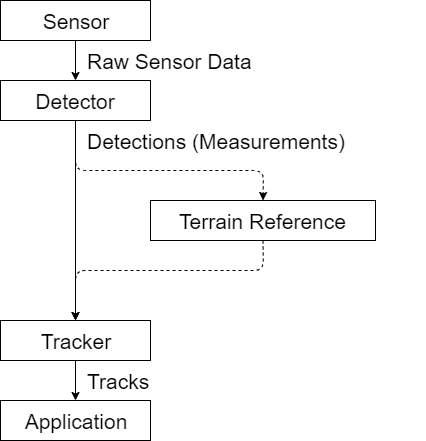
\includegraphics[scale=0.4]{TrackingFlowcharts.png}
    \caption{A tracking framework with optional terrain reference module for terrain-aided tracking}
    \label{fig:trackingflowcharts}
\end{figure}

In \cite{collins1989terrain} a DEM in combination with measurements of the sensor position and orientation are used to add range information to a bearing measurement and then to track the target using a Kalman Filter. Similar strategies are employed in \cite{collins1998using, kim2015utilization, kim2009terrain, mallick2007geolocation, wolfe2002achieving, davison1999mobile, collins2000system, xu2019target, tufan2012emitter}. Figure \ref{fig:lineofsightbasic} illustrates the basic approach of the line of sight algorithms. The line of sight direction is measured by orientation sensors and the sensor position is measured by GPS \cite{collins1989terrain}. Starting from the sensor position the line-of-sight is followed until an intersection with the DEM is reached \cite{collins1989terrain}. The point of intersection in the DEM is used to calculate the range to the target geometrically, and some Gaussian noise (correlated with the angular measurements to the target) is assumed \cite{collins1989terrain}. Derivations for the geolocation estimate and error covariance are given for both a flat earth model and a DEM in \cite{mallick2007geolocation}. These derivations are based on the assumption that sources of error in the geolocation estimate are errors in the sensor position, Euler angles to the target, and terrain height, and these are assumed to be zero-mean and Gaussian \cite{mallick2007geolocation}. 

\begin{figure}[ht]
    \centering
    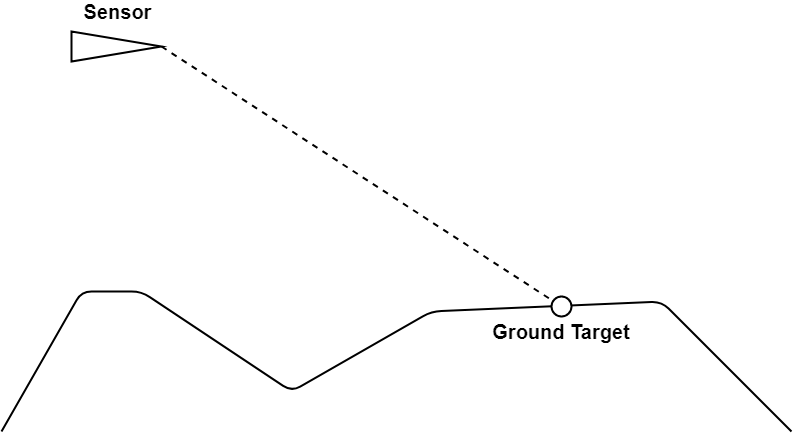
\includegraphics[scale=0.28]{TerrainTrackingDiagram.png}
    \caption{A basic example of line of sight tracking using a digital terrain map}
    \label{fig:lineofsightbasic}
\end{figure}

A limitation of this approach that is identified in the literature \cite{collins1989terrain, collins1998using, davison1999mobile} is the assumption that the distribution of the geolocation measurement (or the augmented range measurement if tracking in spherical coordinates) is Gaussian. In reality situations can arise where there is a multimodal distribution of the target position measurement due to uncertainty in the sensor position, sensor orientation, and errors in the DEM \cite{collins1998using, dastner2009fusion}. These situations can arise due to a low grazing angle or peaky terrain. One such example is illustrated in figure \ref{fig:lineofsightmultimodal} where an error in the DEM can lead to the point of intersection along the line-of-sight being distant from the actual target position. These measurement errors may lead to additional problems in the tracking stage such as reduced track accuracy, broken tracks, track swaps, increased confirmation latency, or formation of multiple tracks for the same target (in multi-target tracking).

\begin{figure}[ht]
    \centering
    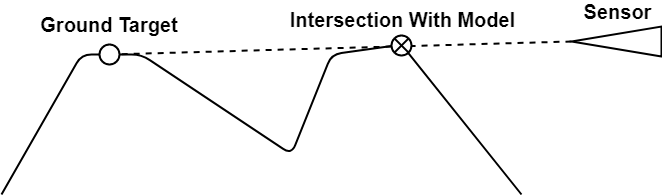
\includegraphics[scale=0.28]{TerrainTrackingDiagramMultimodal.png}
    \caption{Sometimes the distribution of the range measurement noise can be multimodal due to uncertainty in the sensor position, sensor orientation, and DEM}
    \label{fig:lineofsightmultimodal}
\end{figure}

In \cite{kim2009terrain} the unscented transform and Unscented Kalman Filter (UKF) are used to partially address this limitation. The distribution of the target position is still estimated as a Gaussian, which is convenient for integration with existing tracking frameworks, but this still does not capture the possibly multimodal nature of the distribution. The unscented transform yields an error covariance that accounts for the interaction between the measurement errors and the varying terrain height in the area surrounding the measured target position \cite{kim2009terrain}. This is unlike the derivations from \cite{mallick2007geolocation} which only account for the terrain height and its error covariance at the measured target position (where the measurement mean intersects the terrain surface). The method from \cite{kim2009terrain} is very similar to the method described in section \ref{gaussianmodel} and they are expected to produce similar results. The only difference is that in this paper the samples are drawn randomly while in \cite{kim2009terrain} the transformed distribution is computed using sigma points.

Suggestions have been made \cite{collins1998using, davison1999mobile} to use particle-based algorithms such as the CONDENSATION algorithm \cite{isard1996contour} to fully address these limitations but this has not yet been applied to the problem of terrain-aided tracking and may present computational concerns for multitarget tracking scenarios since the total number of particles required may become large. Additionally the CONDENSATION algorithm requires a fully integrated tracking process, often it is desirable to have a model that can be used with tracking processes already in use. This is especially true in this case, since difficult conditions warranting the change may not arise very frequently.

Approaches exist that can improve terrain-aided tracking results using traditional tracking pipelines by selecting an appropriate flight path \cite{barber2006vision}, avoiding conditions likely to cause difficulty. Flight paths cannot always be freely selected however due to flight restrictions or covert operational requirements. Additionally, this strategy has limitations in its ability to track multiple targets since it may not be possible to choose a flight path that is good for all targets.

This paper aims to present an algorithm that can be used to accurately track a target using passive, bearing-only sensors combined with terrain information and measurements of the sensor position and orientation. Additionally, the algorithm presented aims to address the limitations outlined above by presenting a method that is robust to conditions such as low grazing angle, difficult terrain, or having only a low resolution DEM available. When the target position is ambiguous given the available information, the algorithm should be able to recognize this. The algorithm should not depend on a particular choice of flight path, which may be restricted by operational requirements. The algorithm should not prohibit tracking multiple targets. Additionally the algorithm is intended to be applicable for online use in realistic scenarios, so computational requirements should not restrict the algorithm from being used in real time.

This paper proposes to model the measured target position distribution in the terrain-aided tracking problem using a Gaussian mixture model to reflect that the distribution may be multimodal. An algorithm for estimating the parameters of such a model for the case of terrain-aided tracking is presented, using the image processing techniques of dilation and connected component labelling to cluster samples to form the components of the distribution. This mixture model is compared with a Gaussian model in terms of tracking performance through simulation with various DEMs.

The contributions of this paper are as follows. Firstly, an algorithm is proposed to efficiently parameterize a Gaussian mixture measurement distribution for the purposes of terrain-aided tracking measurements. Existing algorithms for this purpose such as Expectation Maximization (EM) or K-Means (KM) require that the number of mixture components is known (which is not practical for terrain-aided tracking since the number of components may vary for different measurements) or involve selecting the best fit over a range of possible numbers of components (which is inefficient and may result in an over-fit). The algorithm presented here can be used to estimate the number of mixture components, addressing this issue and allowing standard methods to be used. Alternatively the algorithm can also be used to cluster samples from the measurement distribution to obtain an estimate of the distribution parameters using simpler methods (based on the sample mean, sample covariance, and weight of each cluster). Secondly, a framework is proposed for the integration of a Gaussian mixture measurement model into existing terrain-aided tracking frameworks using components that are likely to already be in use while requiring minimal modification, and falling back to a standard Gaussian measurement model automatically when appropriate. Lastly, simulation results are provided to assess the performance implications of using a Gaussian mixture measurement model under difficult tracking conditions.

The remainder of the paper is organized into several sections. Section \ref{background} provides background on the subject of digital elevation models, terrain-aided tracking, and multiple hypothesis tracking and outlines the theoretical framework on which this paper builds. Section \ref{problemstatement} provides the mathematical context for the problem under consideration. Section \ref{samplebasedmeasurements} presents the details of the proposed fast algorithm for parameterization of a Gaussian mixture measurement distribution appropriate for use in terrain-aided tracking. In section \ref{simulations} simulated results are presented to compare tracking results using the proposed measurement model against those using a Gaussian measurement model (such as in \cite{kim2009terrain}). Section \ref{conclusion} concludes with a summary, an evaluation of the results from the previous section, identification of limitations of the proposed approach, and directions for future work.








\section{Background} \label{background}

\subsection{Digital Elevation Model (DEM)} \label{digitalterrainmaps}
A Digital Elevation Model (DEM) is a database that can be referenced to obtain an estimate of terrain elevation for a given pair of geographic coordinates (latitude and longitude). DEMs have important applications in Geographic Information Systems (GIS) \cite{qgis} in addition to target tracking and many others. Several different standard representations of DEM are available, but this paper will focus on data represented by a Digital Elevation Matrix. This representation is relatively compact and readily available for public download \cite{jpl13, robinson2012high}. The Digital Elevation Matrix representation is also used for the DTED specification \cite{MILPRF89020B} so its use is common in military applications.

A Digital Elevation Matrix consists of a set of regularly-spaced "posts", each with an estimate of the elevation at that post. Each post is associated with a geographic location in a specified projection, so conversions between geographic and local coordinate systems are possible using standard methods. Between the posts no information about the terrain height is provided, as illustrated by figure \ref{fig:demposts}.

\begin{figure}[ht]
    \centering
    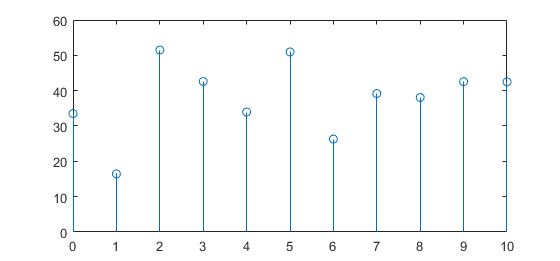
\includegraphics[scale=0.6]{PostsBasic.png}
    \caption{A representation of a single axis of DEM data with elevation measurements provided at post locations and unknown elevations in between}
    \label{fig:demposts}
\end{figure}

The elevation at points between the posts can be approximated by bilinear interpolation of the neighboring 4 posts, which results from \cite{li2005accuracy} suggest provides reasonable accuracy and computational efficiency for this purpose. Therefor the terrain surface modelled by the DEM is a grid of bilinear patches. The equation for such a patch is given in \ref{eq:bilinearpatch}, where $z_W$ is the elevation at a point on the patch, $z_{ij}$ are the elevations provided by the neighboring posts with increments of $i,j$ corresponding to increments in the grid in the $x,y$ directions, respectively.

\begin{dmath} \label{eq:bilinearpatch}
    z_W = w_{y0} (w_{x0} z_{00} + w_{x1} z_{10}) + w_{y1} (w_{x0} z_{01} + w_{x1} z_{11})
\end{dmath}

The weights $w_{x0}, w_{x1}$, $w_{y0}, w_{y1}$ correspond to the distance between the point on the surface and the neighboring posts in the $x$ and $y$ directions respectively for the lower and upper posts (this is just normal bilinear interpolation).

\subsection{Surface Model Intersections} \label{surfaceintersections}
Terrain-aided tracking by line of sight is based on the intersection of the line of sight (a ray from the sensor position in the direction of the target) and the DEM surface, so determining the first point of intersection along this ray will be required for such applications. Since the DEM is a grid of bilinear patches, this task be be divided into a grid traversal over patches in the line of sight and checking each patch for an intersection.

\subsubsection{Ray-Grid Intersection} \label{raygridintersection}
In \cite{collins1998using} the DEM is intersected by traversing the grid cell-by-cell in the $x,y$ coordinates starting from the cell containing the sensor until a point of intersection is found where the elevation in the cell is greater than the $z$ component of the line of sight as it passes through that cell. A Bresenham algorithm suggested for this purpose, but details are not included as to the specific nature of this algorithm.

In \cite{musgrave1988grid} a modified Bresenham Digital Differential Analyzer (DDA) algorithm is presented to traverse a grid along a line. Their algorithm identifies all cells in the grid that intersect the line, and does so in order of intersection from the starting point \cite{musgrave1988grid}, as illustrated in figure \ref{fig:linegrid}. Here the elevation component is also considered, and can be rejected for intersection without an exact intersection test if the elevation of the ray does not pass through the elevation of the cell, otherwise an exact test is performed \cite{musgrave1988grid}.

\begin{figure}[ht]
    \centering
    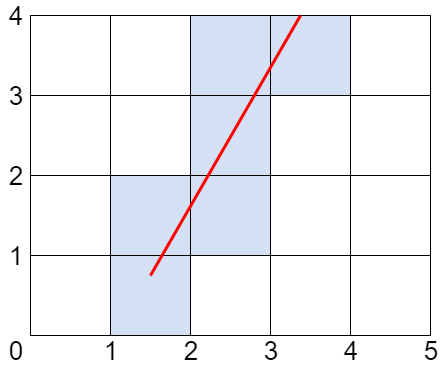
\includegraphics[scale=0.3]{LineGrid.png}
    \caption{An illustration of the cells identified by the modified Bresenham DDA algorithm from \cite{musgrave1988grid}}
    \label{fig:linegrid}
\end{figure}

\subsubsection{Ray-Bilinear Patch Intersection} \label{bilinearpatchintersection}
In \cite{collins1998using} it is suggested to use interpolation to obtain a more precise point of intersection within the intersecting cell, but similarly to the grid intersection method no details are provided. An efficient algorithm for intersecting rays with a bilinear patch is presented in \cite{ramsey2004ray}. A patch may also have multiple intersections, in which case the first (nearest to the sensor) represents the correct point in the line of sight \cite{ramsey2004ray}. This is already considered by the algorithm presented in \cite{ramsey2004ray} which returns the first point of intersection.

\subsection{Gaussian Mixture Models (GMMs)} \label{backgroundgmm}
Mixture models can be used to represent a multimodal distribution as a weighted sum of $K$ component distributions. When the component distributions are all Gaussians then the distribution is called a Gaussian mixture (or a mixture of Gaussians). GMMs are a desirable way to represent multiple hypotheses in a target tracking scenario because they fit conveniently within the frequently-used Bayesian recursive estimation framework for Multiple Hypothesis Tracking (MHT) (see section \ref{backgroundmht}). Equation \ref{eq:gaussianmixture} is the general definition of a Gaussian mixture distribution, where $\mu_i,C_i$ are respectively the mean and covariance of each Gaussian component distribution.

\begin{dmath} \label{eq:gaussianmixture}
    { p(x) = \sum_{i = 1}^K \phi_i \mathcal{N}(\mu_i, C_i) }
\end{dmath}

Various general-purpose approaches exist for estimating a GMM from a set of samples, with two popular types of algorithms being K-means (KM) and Expectation Maximization (EM) \cite{reddy2008trust, umale2014overview, hamerly2004learning}. They are closely related as both are center-based clustering algorithms that involve initializing clusters and updating their centroids based on their relationship with the samples \cite{hamerly2004learning}. KM algorithms cluster the samples based on their Euclidean distance from each cluster centroid (they assigned to the nearest cluster) and use the mean of each cluster's samples to update the centroid for the next iteration, continuing until a stable configuration is reached \cite{umale2014overview}. EM algorithms work in a similar iterative manner, but also consider the probability of each sample's membership to each cluster and may use a more complex distance metric \cite{umale2014overview}. Both algorithms can benefit from good cluster initialization \cite{hamerly2004learning}.

Both KM and EM in their standard forms assume that the number of components is known \cite{hamerly2004learning}. In \cite{hamerly2004learning} an algorithm is proposed to learn the $K$ value in KM, which suggests a method for evaluating the model fit with each choice of $K$. Their algorithm involves $K_{max}$ evaluations of KM \cite{hamerly2004learning}. Assuming a constant number of dimensions the computational complexity of the KM algorithm is $\mathcal{O}(Kni)$ where $K$ is the number of components, $n$ the number of samples, and $i$ the number of iterations \cite{hartigan1979algorithm}. If $K_{max}$ iterations are performed to determine $K$ then then total computational complexity is $\mathcal{O}(K_{max} K n i)$. This complexity may be prohibitive for real time use in tracking applications where a high frame rate is required when $K_{max}$ is large. Additionally it is possible that the resulting mixture with the best fit may involve an excessive number of components that do not correspond well to different hypotheses in a tracking context (see section \ref{kclusters}). Section \ref{gaussianmixturemodel} of this paper proposes an alternative method to approximately cluster samples and determine the a reasonable number of components to use in the context of terrain-aided tracking.

\subsection{Multiple Hypothesis Tracking (MHT)} \label{backgroundmht}
In \cite{kim2015multiple} it is demonstrated that Multiple Hypothesis Tracking (MHT) can be an effective method for resolving ambiguities in visual tracking problems. With MHT the final decision on data association is delayed by maintaining a tree of all hypotheses originating from a particular observation, though in practice this tree must be pruned aggressively for MHT to remain computationally feasible \cite{kim2015multiple}. In each frame the tree is updates as each hypothesis is associated with new observations as well as a dummy observation (indicating a missed detection) \cite{kim2015multiple}. The most likely global hypothesis at each frame is then formed with the constraint that each observation is either a false alarm or associated with a single track (i.e. there are no unresolved targets).

The relevant aspects of approaches from \cite{kim2015multiple, li2013multitarget, yamada2017multi} are reviewed below. These approaches all utilize MHT for multi-target tracking. Additionally \cite{li2013multitarget, yamada2017multi} use MHT to resolve ambiguities with the measurement distribution (in terms of Doppler measurements and grating lobes). The same approach will be applied in this paper to resolve ambiguity in terms of the Gaussian mixture measurement modes as well as in measurement-to-track association (for multi-target tracking) without much modification. In \cite{kim2015multiple} a visual appearance model is also used during association, this will not be reviewed here as this paper does not assume this information is available from the sensor.

\subsubsection{Track Trees}
In MHT the track hypotheses originating from each observation are represented by track trees, constructed each frame for every observation (detection) to consider the possibility that new targets are being observed \cite{kim2015multiple}. In subsequent frames these trees are updated by adding hypothesis branches with increasing depth corresponding the different possible association outcomes originating from the root observation of each tree \cite{kim2015multiple}. In a particular tree each directed path from the root to a leaf of the tree is one hypothesis corresponding to the initial observation (the root). These hypotheses are each given a track score, which is used in pruning the tracks as well as computing the global track hypothesis \cite{kim2015multiple,li2013multitarget,yamada2017multi}. The track tree can be pruned based on an N-scan approach as well as kept to a maximum number of branches to keep computation feasible \cite{kim2015multiple}. The N-scan approach involves looking back N frames in the tree and pruning branches that are not in the current global hypothesis \cite{kim2015multiple}. The maximum size can be enforced by keeping only the top hypotheses based on their track scores \cite{kim2015multiple}. Additional logic-based (i.e. "M out of N") or score-based track management can be employed to confirm or terminate tracks.

At each frame existing tracks are updated to account for new observations of objects which have been previously observed as well as missed observations \cite{kim2015multiple}. To consider objects that have been observed before existing track hypotheses (in all trees) are updated by appending a new branch for each new observation that lies within their gating region \cite{kim2015multiple}. New observations are said to be within the gating region for a track hypothesis if the Mahalanobis distance between the observed location and the location predicted by the hypothesis is less than a specified threshold \cite{kim2015multiple}. This is seen in equation \ref{eq:mahalanobis} (from \cite{kim2015multiple}) where $d_{M}$ is the Mahalanobis distance between the predicted hypothesis (with mean $\mu_x$ and covariance $\Sigma_x$ obtained using a Kalman filter) and the observed location $\mu_y$. The threshold can be adjusted to increase or decrease the size of the gating region \cite{kim2015multiple}. This gating procedure reduces the total number of hypotheses to consider.

\begin{dmath} \label{eq:mahalanobis}
    { d_{M} = (\mu_x - \mu_y)^T (\Sigma_x)^{-1} (\mu_x - \mu_y) }
\end{dmath}

In \cite{li2013multitarget,yamada2017multi} this gating test based on Mahalanobis distance is applied for all combinations of existing hypotheses with each ambiguous case (i.e. the Doppler measurement or grating lobe) from all new measurements and a new hypothesis is formed for each combination passing the test. In the standard MHT \cite{kim2015multiple}, each measurement generates only one hypothesis to test per existing hypothesis, while in the formulations from \cite{li2013multitarget,yamada2017multi} each measurement generates one or more hypotheses to test for each existing hypothesis.

In \cite{li2013multitarget} an equation for the probability of each hypothesis is derived using Bayes' theorem, repeated here in equation \ref{eq:hypothesisprobability}. The first factor in the product correspond to the measurements' likelihood (including the Doppler measurement) given the hypothesized association \cite{li2013multitarget}. The second factor is the probability of the current hypothesis given the previous one, which includes both the measurement-to-track assignment and the Doppler order assignment \cite{li2013multitarget}. The final factor is the probability of the parent hypothesis, and $c$ is a normalization constant chosen so that the sum of the probabilities for all hypotheses is $1$.

\begin{dmath*} \label{eq:hypothesisprobability}
    P\{A^{k,l}|Z^{k}\} = \penalty0
    \frac{1}{c} \penalty0
    p[ Z(k) \given[\Big] a(k), A^{k-1,s}, Z^{k-1} ] \penalty0
    \cdot P\{a(k) \given[\Big] A^{k-1,s}, Z^{z-1} \} \penalty0
    \cdot P\{ A^{k-1,s} \}
\end{dmath*}

A simplified final expression is repeated below (equation \ref{eq:hypothesisprobabilitysimp}), also from \cite{li2013multitarget}. The probability depends on the number of new measurements $m(k)$, number of associated measurements $N_D$, number of false alarms $N_{NF}$, density of new measurements or clutter $\mu_{n+f}$, the number of existing targets $N_{TGT}$, probability of detection $P_D$, tracking volume $V$, and the likelihood of each the of the measurements given the hypothesis $f_{ti}(\cdot)$ (Kalman filter innovation PDF) \cite{li2013multitarget}. More details are given in \cite{li2013multitarget}.

\begin{dmath*} \label{eq:hypothesisprobabilitysimp}
    P\{A^{k,l}|Z^{k}\} = \penalty0
    \frac{N_{D}!}{c \cdot m(k)!} \penalty0
    \mu_{n+f} \penalty0
    \cdot P^{N_D}_D \penalty0
    \cdot (1 - P_D)^{N_{TGT}-N_{D}} \penalty0
    \cdot V^{-N_{NF}} \penalty0
    \cdot { \prod_{i \in a_{T}(k)}^{m(k)} f_{ti}(Z_i^U,k) }
\end{dmath*}

In the derivation from \cite{li2013multitarget} the Doppler distribution is assumed to be uniform so its contribution is absorbed into the normalization constant $c$. However in \cite{yamada2017multi} some information about the strengths of the possible grating lobes is considered here. Since this distribution is no longer uniform, an additional factor is added to the equation. This factor corresponds to the weight of the lobe for the lobe hypothesis in \cite{yamada2017multi}, but can also be the weight $\phi_i$ from a Gaussian mixture component to hypothesize about different modes.

\subsubsection{Global Hypothesis}
Forming a global hypothesis is achieved by determining the most likely set of compatible tracks based on all of the the current hypotheses. As described in \cite{kim2015multiple}, the formation of a global hypothesis is equivalent to solving the Maximum Weight Independent Set (MWIS) problem on a graph with nodes for each hypothesis and edges between nodes which are in conflict. Solving this problem is equivalent to solving the Maximum Weight Clique problem on the complement graph (with the same nodes, but edges instead connecting nodes which are compatible). The Maximum Weight Clique problem can be solved using a number of different exact or approximate algorithms, and the simulations in this paper use the algorithm from \cite{ostergaard2001new}. When considering track compatibility, a pair of tracks will be considered incompatible if they both involve the association of the same measurement (multiple targets cannot originate from a single measurement) \cite{kim2015multiple,li2013multitarget,yamada2017multi}.

\subsection{Morphological Image Processing} \label{morphological}
In \cite{ravankar2015connected} morphological image processing techniques were used with sparse Lidar data to segment the data points. Their goal was to find structures (walls) in the surrounding area but binning and the segmenting the Lidar data directly using Connected Component Labeling (CCL) led to incorrect clustering due to the sparse nature of the data points \cite{ravankar2015connected}. This was addressed by applying a dilation to the bin map before clustering using CCL \cite{ravankar2015connected}. This technique will be applied

\subsubsection{Dilation}
Dilation expands existing pixels in a binary image with values of $1$ so that their neighboring pixels also have values of $1$. The region of pixels to be considered as neighbors can be defined by specifying a structuring element matrix \cite{ravankar2015connected}. By enlarging these regions in the image, nearby regions may join one another, and this is how the data sparsity issue is addressed in \cite{ravankar2015connected}. See figure \ref{fig:connectedcomponents} showing the effects of dilation on CCL as applied in this paper.

\subsubsection{Connected Component Labeling}
Connected Component Labeling (CCL) is used to label clusters of pixels with values of $1$ in a binary image that are connected. Pixels are considered connected if a path exists between them of adjacent pixels with values of $1$ according to some neighbor relation (usually 4-way or 8-way). Each pixel is assigned a label such that pixels sharing the same label belong to the same connected component. See figure \ref{fig:connectedcomponents} for an example of labeled connected components (with and without dilation). A review of conventional CCL algorithms as well as a faster algorithm can be found in \cite{he2009fast}. This map of labels is used in \cite{ravankar2015connected} to cluster the data points.









\section{Problem Statement} \label{problemstatement}
Ground point targets moving through rough terrain are tracked using a passive sensor from an airborne platform equipped with sensors to measure its own orientation and position. The platform is also equipped with a Digital Elevation Model (DEM) of the tracking area. The information from these sources will be used to estimate the distribution of the position of the detected object based on the method proposed in section \ref{samplebasedmeasurements}.

\subsection{Assumptions} \label{probstatementassumptions}
The sensor is assumed to be able to measure its own position and the angles to the targets (elevation and azimuth) with zero-mean Gaussian noise. The DEM is assumed to provide the correct elevation for a given set of geographic coordinates, though this is not the case in reality (the effect of this assumption is investigated by considering simulation results using multiple DEMs with varying resolution and accuracy in section \ref{simulations}).

Multiple targets are considered in the tracking stage, but this paper focuses on modeling the terrain-aided detection distribution so at this stage the targets are considered individually based on the assumption of a one-to-one correspondence between targets and true measurements (no unresolved targets, no extended targets).

\subsection{Reference Coordinates}
The targets are tracked in the local frame of reference, that of the DEM, with units in meters. Conversions back and forth between the local frame of reference and geographic coordinates are straightforward using standard tools (see section \ref{digitalterrainmaps}). These conversions are necessary for practical applications, for example to bring tracking information back to geographic coordinates for the end use application. They are used for the simulations discussed in section \ref{simulations}.

\subsection{Scenario}
A target located at position $X_T$ is observed by a sensor located at position $X_S$ with viewing direction vector $D_T$ (a unit vector in the direction of the line between the sensor and the target). 3 dimensions are being considered.

\begin{dmath}
    X_T = [x_T, y_T, z_T]^T
\end{dmath}
\begin{dmath}
    X_S = [x_S, y_S, z_S]^T
\end{dmath}
\begin{dmath}
    D_T = [x_D, y_D, z_D]^T
\end{dmath}

The target is a ground point target so its position lies on the terrain surface. The elevation of the terrain is represented by the function $z_{W}(x,y)$, corresponding to the DEM (see section \ref{digitalterrainmaps} for details).

\subsection{Sensor Measurements}
As assumed (see section \ref{probstatementassumptions}) the sensor measurement PDF is given by equation \ref{eq:sensormeasurementvector}. Where $Z_S$ is the sensor measurement vector and $C_S$ is the sensor measurement noise covariance matrix. Note that here the angle to the target is measured in terms of azimuth $\theta_T$ and elevation $\varphi_T$ so the measurement noise is Gaussian in those variables.

\begin{dmath} \label{eq:sensormeasurementvector}
    Z_S = [x_S, y_S, z_S, \theta_T, \varphi_T]^T + \mathcal{N}(0, C_S)
\end{dmath}

Intuitively the sensor is measuring the line of sight to the target. The measured variables are combined to form the line of sight $L$ in equation \ref{eq:lineofsightrv} where $t$ is a free parameter that moves along the line. Here $D_T$ is obtained through the standard Spherical to Cartesian conversion.

\begin{dmath} \label{eq:lineofsightrv}
    L = X_S + t D_T
\end{dmath}

Figure \ref{fig:measurementrvs} shows samples from the distribution of $L$ which represent possible lines of sight based on the information from the sensor measurements.

\begin{figure}[H]
 \centering
 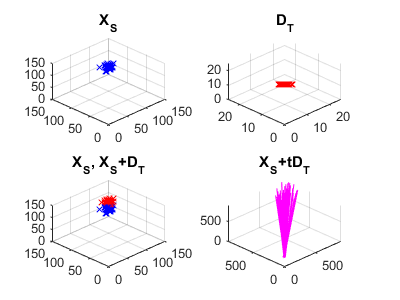
\includegraphics[scale=0.8]{measurementrvs.png}
 \caption{Samples from the distributions of random variables related to the line of sight from the sensor to the target. Here the sensor measurements have zero-mean white Gaussian noise.}
 \label{fig:measurementrvs}
\end{figure}

\subsection{Target Motion Model}
The methods proposed in this paper are not influenced by the choice of target motion model, so any motion model can be used. A constant velocity model with process noise is used in the simulations presented in section \ref{simulations} but this is selected purely for ease of implementation. The proposed method involves a multimodal measurement model, but this measurement is then split into several Gaussian hypotheses for Multiple Hypothesis Tracking as described in section \ref{backgroundmht}. The affect of this in the tracking stage is that the number of hypotheses is increased, but each individual hypothesis can still be tracked in the normal way. This approach allows for target state predictions to be evaluated in the normal way with respect to the target motion model. Maneuvering targets could also be handled in this way with minor modifications to existing methods based on IMM-MHT (such as in \cite{liu2019multiple}) through the introduction of additional hypotheses generated by each component of the measurement.








\section{Sample-Based Terrain-Aided Measurements} \label{samplebasedmeasurements}
In \cite{kim2009terrain} a UKF is used for Terrain-aided tracking, which involves obtaining samples from the target position distribution, and the same basic strategy is employed here to obtain such samples. First samples are drawn from the distribution of the sensor measurements, then these samples are interpreted as lines of sight and transformed by intersecting them with the terrain model. This process is described in detail below and suggestions are made for specific intersection algorithms to use for this transformation.

These samples are then used to parameterize an estimate of the target position distribution. In \cite{kim2009terrain} this distribution is estimated as a Gaussian, and a similar method is included here first as a base of comparison with no novelty claimed. This paper then proposes to model the target position distribution as a Gaussian mixture and presents an algorithm based on morphological image processing to cluster the samples and estimate the number of mixture components in the case of terrain-aided tracking. Two alternatives are then given to compute the final mixture parameters once the clustering is completed. The sampling process does not account for uncertainty in terms of the elevation values provided by the DEM. To alleviate this, some additional variance is added in the $z$ direction.

\subsection{Sample Representation} \label{particlemodel}
Here the goal is to obtain a set of samples from the distribution of the target position given the information from the sensor measurement and the DEM. A set of $n$ samples $s_i$ are drawn from the distribution of $L$ (equations \ref{eq:samplei} through \ref{eq:dssample}). Each sample represents a possible line of sight from the sensor to the target. Let $L^*$ be the set containing these samples as in equation \ref{eq:lossampleset}. These line of sight samples are visualized in figure \ref{fig:measurementrvs} from the previous section.

\begin{dmath} \label{eq:samplei}
    i \in 1,\ 2,\ ..,\ n
\end{dmath}
\begin{dmath} \label{eq:lossample}
    {l_i = x_i + t d_i}
\end{dmath}
\begin{dmath} \label{eq:xssample}
    {x_i \leftarrow X_S}
\end{dmath}
\begin{dmath} \label{eq:dssample}
    {d_i \leftarrow D_T}
\end{dmath}
\begin{dmath} \label{eq:lossampleset}
    {L^* = \{ l_1,\ l_2,\ ..,\ l_n\}}
\end{dmath}

The target is assumed to be a ground point target, so the target position is the nearest location to the sensor where the line of sight intersects with the terrain surface. Sample points of intersection $p_i$ are therefor given by equation \ref{eq:possample}. 

\begin{dmath} \label{eq:possample}
    {s_i = x_i + t_i d_i}
\end{dmath}

In the above $t_i$ is chosen as the minimum positive $t$ value (in front of the sensor) where the sample line $l_i$ intersects the terrain surface $X_w$. This is expressed as an optimization problem in equation \ref{eq:mint}.

\begin{subequations}\label{eq:mint}
\begin{alignat}{2}
&\!\min_{t}          &\qquad& t\\
&\text{subject to} &      & x_i + t d_i = X_w,\\
&                  &      & t > 0
\end{alignat}
\end{subequations}

Recall that the world surface $X_w$ is modelled as a grid of bilinear patches. The algorithm presented in \cite{ramsey2004ray} and reviewed in section \ref{bilinearpatchintersection} can be applied to find the point of intersection with the minimum $t$ for each bilinear patch. Because the DEM has a finite number of patches it is possible in theory to find the minimum $t$ in equation \ref{eq:mint} by searching each patch in the DEM to determine all possible values of $t$ that meet the constraints and then selecting the smallest one. Such an approach presents obvious potential computational concerns if the DEM is large so it is desirable to avoid searching every patch.

Patches of interest are those that intersect the ray in the $x,y$ coordinates, as seen in figure \ref{fig:linegrid} where the grid is numbered in post coordinates in the $x,y$ axes (points of intersection on the grid are at post locations). Let patch $i,j$ be the bilinear patch between posts $i,j$ and $i+1,j+1$. The $x,y$ coordinates of the ray starting point are converted to pixel coordinates for the purposes of grid traversal, as in equation \ref{eq:linepixelcoords} where $s_{pixel}$ is the pixel size (DEM post spacing or resolution) in meters.

\begin{dmath} \label{eq:linepixelcoords}
    {[x_{pixel}, y_{pixel}] = [x_{local} / s_{pixel}, y_{local} / s_{pixel}]}
\end{dmath}

The sample ray in pixel coordinates is then intersected with the DEM at the cell level using the algorithm presented in \cite{musgrave1988grid} and described in section \ref{raygridintersection} to determine candidate cells. Each of the candidate cells are tested for exact intersection as described in section \ref{bilinearpatchintersection} until a true intersection is found. Since only the nearest point of intersection for each line is required the process can be stopped when one is found. This method is used for each line of sight sample $l_i$ in $L^*$.

Each sample $s_i$ represents one possible target location relative to the global coordinates. Let $S^*$ be the set containing these samples as in equation \ref{eq:possampleset}. These samples will be used to estimate the distribution of the target position.

\begin{dmath} \label{eq:possampleset}
    {S^* = \{ s_1,\ s_2,\ ..,\ s_n\}}
\end{dmath}

\subsection{Gaussian Model} \label{gaussianmodel}
Once samples $S^*$ of the target position are generated as in section \ref{particlemodel} a Gaussian approximation of the distribution can be formed. This can be done by taking the sample mean and sample covariance of $S^*$. The sample mean is computed by equation \ref{eq:possamplemean}. The sample covariance matrix is computed by equation \ref{eq:possamplecov} where $F$ is a matrix with rows corresponding to the $x,y,z$ components of the samples and the columns corresponding to the samples (as in equation \ref{eq:possamplematrix}). This is very similar to the method from \cite{kim2009terrain} where the unscented transform is used, and will be used as base of comparison.

\begin{dmath} \label{eq:possamplemean}
    {\mu_p = \frac{1}{n} \sum_{i = 1}^n s_i}
\end{dmath}
\begin{dmath} \label{eq:possamplecov}
    {C_p = \frac{1}{n - 1} (F - \mathbf{1}_n \mu_p^T) (F - \mathbf{1}_n \mu_p^T)^T }
\end{dmath}
\begin{dmath} \label{eq:posonesvec}
    {\mathbf{1}_n = [\underbrace{1,\ 1,\ ..,\ 1}_{n\text{-times}}]}
\end{dmath}
\begin{dmath} \label{eq:possamplematrix}
    {F = [s_1,\ s_2,\ ..,\ s_n]}
\end{dmath}

\subsection{Gaussian Mixture Model} \label{gaussianmixturemodel}
Similarly to the Gaussian model, the samples taken as in section \ref{particlemodel} are again used to approximate the measurement distribution, but this time modeling the distribution with a multivariate Gaussian Mixture model. The distribution for this model is given in equation \ref{eq:sbgmm} where $K$ is the number of components of the mixture model and $\phi_i, \mu_i, C_i$ are respectively the weight, mean, and covariance matrix corresponding to each mixture component indexed by $i$ (see section \ref{backgroundgmm}).

\begin{dmath} \label{eq:sbgmm}
    { p(x_T) = \sum_{i = 1}^K \phi_i \mathcal{N}(\mu_i, C_i) }
\end{dmath}

To form this distribution it will be necessary to determine the number of components $K$, and then estimate the weight, mean, and covariance matrix for each component. A method is proposed below to cluster the samples into sub-populations for formation of a Gaussian mixture while simultaneously estimating for the number of components $K$. Once the samples are clustered, the samples from each cluster will be used to estimate the parameters for one component of the Gaussian Mixture.

\subsubsection{Approximate Clustering and Determination of the Number of Components} \label{kclusters}
The clusters can be formed by partitioning the $x,y$ space, with each sample assigned to a unique cluster based on its position in $x,y$ coordinates. During the sampling process described in section \ref{particlemodel} a binary mask $M$ the same size as the DEM is produced. When each sample is taken, the mask pixel corresponding to the DEM cell where the intersection occurred is set to $1$. This relationship is expressed in equation \ref{eq:clustermask}. In this equation $s_{pixel}$ is the sample converted to pixel coordinates, which is then floored to yield its integer cell coordinates in the DEM.

\begin{dmath} \label{eq:clustermask}
    M_{x,y} = \begin{cases}
        1 & \exists s \in S^*\ \text{where}\ \lf s_{pixel} \rf = [x,y] \\
        0 & otherwise \\
    \end{cases}
\end{dmath}

Figure \ref{fig:intersectionmask} shows an example of such a binary mask. While the DEM can be quite large, most of the values in the mask will be zero for realistic measurements. Therefor to save memory and computation time the mask $M_{x,y}$ can be represented as a sparse matrix where only cells containing non-zero values are actually stored.

\begin{figure}[ht]
    \centering
    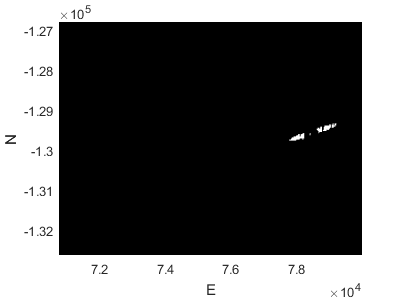
\includegraphics[scale=0.75]{intersectionmask.png}
    \caption{Binary mask of the DEM cells that contain points of intersection, only a small portion of the full size DEM is shown here but with a sparse representation only non-zero values are stored}
    \label{fig:intersectionmask}
\end{figure}

A two-pass connected-component labelling algorithm is applied to this mask to cluster the DEM cells. By using a sparse matrix representation of the mask it is possible to avoid iterating over the whole size of the DEM, only mask cells with non-zero values and their neighbors need to be considered which drastically reduces the total computation time.

\begin{figure}[ht]
    \centering
    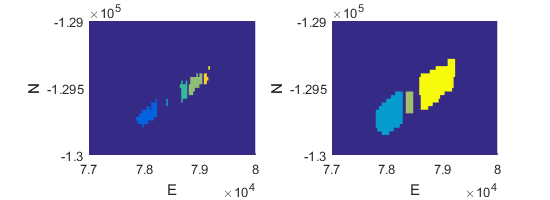
\includegraphics[scale=0.65]{components.png}
    \caption{DEM cells containing points of intersection, clustered by connected component labelling with no dilation (left) and with dilation using a 5x5 structuring element matrix of ones (right)}
    \label{fig:connectedcomponents}
\end{figure}

Depending on the sample density and pixel size of the DEM this may result in a large number of clusters being formed. This is not desirable from a computational perspective since each cluster will form a hypothesis that must be considered for tracking. Therefor clusters that are close together are merged to reduce the overall number of components. This can be achieved through binary image dilation of the mask $M$ before the clusters are formed, as seen in figure \ref{fig:connectedcomponents}. Here through direct labeling 6 components are found, but with dilation applied first several components are merged resulting in only 3 components. This addresses data point sparsity in connected component labeling the same way as in \cite{ravankar2015connected}, as reviewed in section \ref{morphological}.

\subsubsection{Gaussian Mixture Parameterization Using Cluster Sample Mean and Sample Covariance} \label{gmmparamsmsc}
After approximate clustering, each of the $K$ components of the Gaussian mixture can be parameterized using samples from each of the $K$ clusters using a the same method that was use for a single Gaussian in section \ref{gaussianmodel}. That is, the mean and covariance for each component are estimated using the sample mean and sample covariance for the samples in the corresponding cluster as in equations \ref{eq:componentsamplemean} and \ref{eq:componentsamplemean}. Here $F_i,\mathbf{1}_{m_i}$ are defined as in section \ref{gaussianmodel} (but using the samples from cluster $i$), the $m_i$ are the numbers of samples in each component (cluster) $i$, and the $s_j$ are the corresponding samples in that component with $j \in \{ 1,2,..,m_i \}$. To complete the formation of the Gaussian mixture it is also necessary to determine the weight for each component. Here each component is weighted according to the relative frequency of samples occurring in that component, as in equation \ref{eq:componentweight}. This guarantees that the sample weights $\phi_i$ will sum to $1$ as is required for a mixture model.

\begin{dmath} \label{eq:componentsamplemean}
    {\mu_i = \frac{1}{m_i} \sum_{j = 1}^{m_i} s_j}
\end{dmath}
\begin{dmath} \label{eq:componentsamplecov}
    {C_i = \frac{1}{m_i - 1} (F - \mathbf{1}_{m_i} \mu_p^T) (F - \mathbf{1}_{m_i} \mu_p^T)^T }
\end{dmath}
\begin{dmath} \label{eq:componentweight}
    \phi_i = \frac{m_i}{n}
\end{dmath}

One downside of this approach is that some of the clusters may have a small number of samples. This increases the likelihood that the computed sample covariance matrix is not positive-definite, resulting in a non-invertible innovation covariance matrix during tracking. Inversion of the innovation covariance matrix is required to compute the Kalman gain during the update stage, so clusters with a small number of samples may need to be discarded. The overall chance of this occurring can be reduced by increasing the number of samples used, but this may be undesirable for due to the increased computational load it would incur.

\subsubsection{Gaussian Mixture Parameterization Using Expectation Maximization} \label{gmmparamem}
As identified in section \ref{backgroundgmm}, Expectation Maximization is a well-established algorithm for parameterization of a Gaussian Mixture distribution. The main drawback of this approach is that the number of components $k$ needs to be known, or multiple parameterizations must be compared based on some fitment criteria to choose the best. By first applying the algorithm proposed in section \ref{kclusters} to estimate the number of components and then applying a standard EM algorithm a parameterization appropriate for terrain-aided tracking can be obtained. Here the term appropriate is used in the sense that the resulting Gaussian mixture distribution should not have an excessive number of components, and these components should be well-spaced so as to form relatively distinct hypotheses for the target location. The advantages of dynamically selecting a reasonable value for the number of components, compared with selecting a fixed value for $k$ that may be too large, are illustrated through experimental results in section \ref{simulations}.

% \subsubsection{Computational Complexity}
% Due to the real-time requirements of many tracking applications, computational complexity is an important consideration for any practical algorithm. Therefor the proposed algorithm for GMM parameterization is compared to alternatives, Expectation Maximization (EM) and K-Means (KM), in terms of asymptotic complexity. EM and KM both have a computational complexity of $\mathcal{O}(NKDI)$ where $N$ is the number of data points, $K$ is the number of clusters (components), $D$ is the number of dimensions, and $I$ is the number of iterations performed \cite{zhang1999k}.

% For EM and KM algorithms the number of iterations $I$ depends highly on the specific algorithm's convergence properties, but it will of course be at least 1. The proposed algorithm is non-iterative and therefor its computational complexity does not depend on $I$. For the problem of terrain-aided tracking, the number of dimensions $D$ for a naive application of the algorithm is the 3 spatial dimensions, however the proposed algorithm takes advantage of the fact that the samples lie on a surface and performs clustering in 2 only spatial dimensions. These are all constants however, and the analysis here is performed in terms of asymptotic complexity. Therefor the dimension component will not be considered and the computational complexity of EM and KM algorithms under consideration can be given as $\mathcal{O}(NKI)$.

% The proposed algorithm can be decomposed up into three stages. First the binary mask is created indicating cells in the DEM where samples are located in the XY-plane. Next, then the mask is converted into a label mask through connected-component labelling. Finally, the samples are binned using the label mask. The total asymptotic clustering time is the sum of the computational time for each of the stages, as expressed in equation \ref{eq:bigocluster}.

% \begin{dmath} \label{eq:bigocluster}
%     \mathcal{O}_{cluster} = \mathcal{O}_{mask} + \mathcal{O}_{label} + \mathcal{O}_{bin}
% \end{dmath}

% Creating the binary mask involves a constant-time marking operation for each sample, including dilation if the number of dilations is assumed to be constant. Therefor creation of the mask depends only linearly on the number of samples, so its asymptotic computational complexity is $\mathcal{O}(N)$.

% Labeling of the connected components in the binary mask (image) is accomplished using a two-pass connected component labeling algorithm. Many such algorithms exist with computation time $\mathcal{O}(p)$ where $p$ is the number of pixels in the image \cite{wu2009optimizing}. Since a sparse representation of the binary mask is used (see section \ref{kclusters}), and two-pass algorithms only require action at marked pixels of the binary mask, $p$ will be a constant multiple of $N$. These algorithms store the equivalence relation between labels using a union-find data structure, which can take up to $K$ total constant-time operations, but since $K \leq N$ this does not affect the asymptotic complexity. Therefor the labeling stage also has an asymptotic complexity of $\mathcal{O}(N)$.

% Lastly each sample must be binned. For each sample this operation is constant since it is effectively implemented as a lookup table on the label mask constructed in the previous step. Again this stage has an asymptotic complexity of $\mathcal{O}(N)$.

% Combining computation time of the three stages and forgetting about the constant factor of 3 shows that the proposed algorithm's computation time depends asymptotically only linearly on the number of samples $N$ (equation \ref{eq:bigoclusterfinal}).

% \begin{dmath} \label{eq:bigoclusterfinal}
%     \mathcal{O}_{cluster} = \mathcal{O}(N)
% \end{dmath}

% It is also worth noting that both EM and KM require the number of components $K$ to be known or estimated either before applying the algorithm, or through selection of the best fitting parameterization after multiple runs of the algorithm \cite{pham2005selection}. In the case of terrain-aided tracking $K$ can vary with each measurement, so this parameter would need to be estimated. This is a clear advantage of the proposed method, in that $K$ is estimated automatically at the same time as clustering. The approach employed by the proposed algorithm is similar to the visualization approach described in \cite{pham2005selection}, but it is employed while clustering instead of prior to clustering (via KM or EM). The magnitude of the difference in computation time depends on the method chosen to select $K$, but in any case this factor would favor the proposed algorithm since this step is not required at all.






\section{Simulations} \label{simulations}
Simulations were conducted to evaluate the performance of different tracking methods in a variety of tracking conditions. These simulations had two main objectives. The first objective was to compare the the proposed alternatives against a baseline Gaussian model. The second was to assess the effects of elevation model quality on the tracking results, and to accomplish this simulations with a total of 4 DEMs of varying resolution and accuracy were performed. Each configuration was tested over 5000 Monte Carlo runs in a scenario with a single sensor tracking two targets moving through rough terrain. Performance was evaluated in terms of track accuracy, number of false tracks, track completeness, and computation time. False alarms (uniform randomly distributed in tracking frame) and missed detections are included.

\subsection{Tracking Methods Compared}
These simulations include results from four different tracking methods to be compared. The baseline method uses a Gaussian distribution to model the target position measurements, as described in section \ref{gaussianmodel}. The rest of the methods evaluated all model the measurement using a Gaussian mixture distribution, but use different methods to parameterize the distribution. Two of these methods use the approximate clustering method to estimate the number of mixture components described in section \ref{kclusters}, one of which (GMM-DK-SMC) then parameterizes the components by the cluster sample means and sample covariances, while the other (GMM-DK-EM) uses Expectation Maximization (EM) for this purpose. The final method being evaluated (GMM-K6-EM) uses EM with 6 mixture components, an over-fit of the measurement distribution under most circumstances. The open source EM implementation used in these simulations is described in detail in \cite{sanderson2017open}. Figure \ref{fig:sample_frame} illustrates how each of the measurement distributions under consideration compares with the distribution of the samples from the measured target position distribution during difficult tracking conditions. The samples from each of the measurement distributions using a GMM look similar at first glance, but as discussed in section \ref{results} the differences (particularly in terms of the number of mixture components) can affect tracking performance.

\begin{figure}[ht]
    \centering
    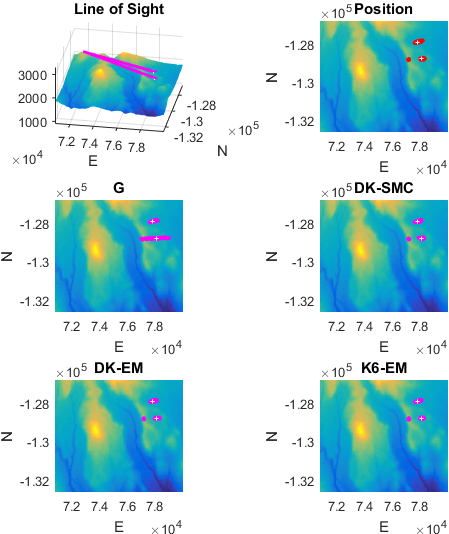
\includegraphics[scale=0.7]{sample_frame.png}
    \caption{Samples from the measurement distribution transformed to their corresponding line of sight and target position samples (top row), and from the measurement distributions assumed when using the four different tracking methods (middle and bottom rows). In each plot the true target positions are marked in white.}
    \label{fig:sample_frame}
\end{figure}

\subsection{DEMs of the Area Surrounding Crater Lake}
Crater Lake (Oregon, USA) was selected as the simulation region because it met several criteria. The area has ample terrain capable of introducing the challenges identified in section \ref{introduction}. Additionally a high resolution DEM is publicly available to be used as the terrain ground truth \cite{robinson2012high}, as well as several lower-resolution DEMs \cite{jpl13, nasa00} more typical of what might be available for general tracking use in various locations around the world. To investigate the effects of DEM accuracy and resolution on tracking performance several compound DEMs were also created to compare based on the above mentioned DEMs. All the DEMs used are described below.

\subsubsection{DEM with 1m Resolution (Ground Truth)} \label{dem1m}
A high resolution DEM of the simulation area is publicly available \cite{robinson2012high}. Created using LIDAR, this DEM has a resolution (post spacing) of 1 meter \cite{robinson2012high}. Figures \ref{fig:craterlake_1m} and \ref{fig:craterlake_1m_zoom} show QGIS \cite{qgis} renderings of the high resolution DEM both in overview and to demonstrate the level of detail. This DEM is used as the ground truth due to its significantly higher resolution than those available for much of the world. It is used to generate the true sensor and target trajectories, and to determine if the sensor has a line of sight to the target. Here it is assumed that the DEM with 1m resolution is acceptably close to the true terrain for the purposes of performance evaluation.

\begin{figure}[ht]
    \centering
    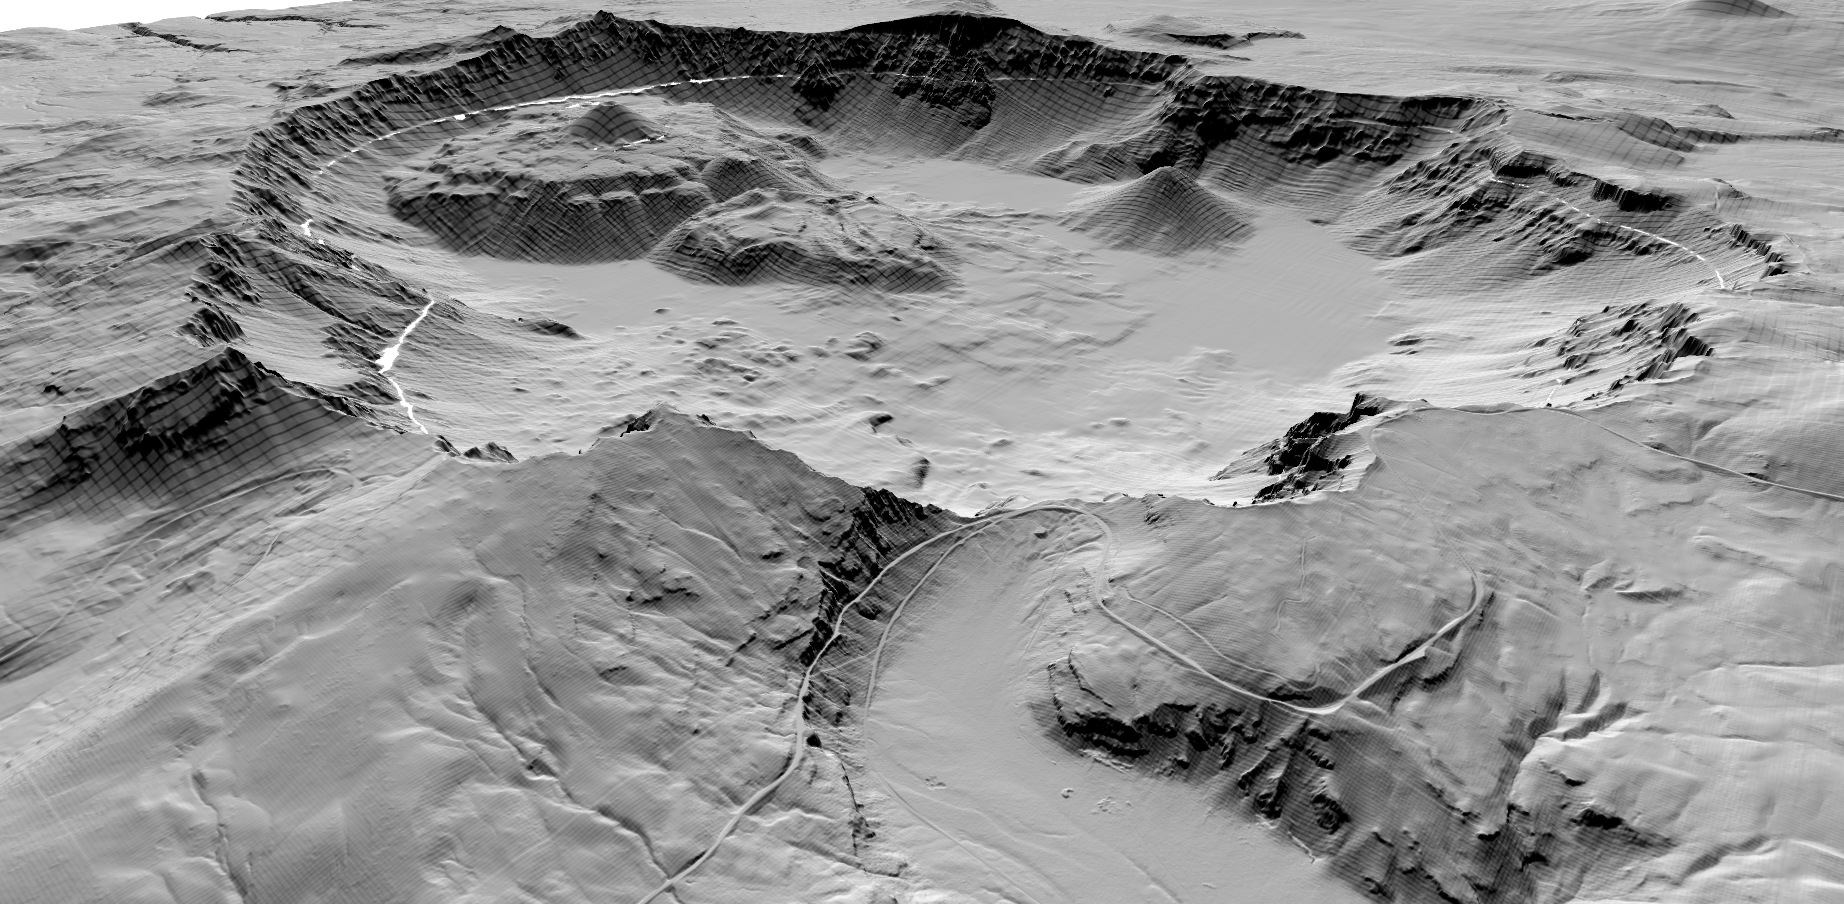
\includegraphics[scale=0.15]{craterlake_highres.png}
    \caption{Challenging terrain surrounding Crater Lake visualized using the DEM with 1m resolution}
    \label{fig:craterlake_1m}
\end{figure}

\begin{figure}[ht]
    \centering
    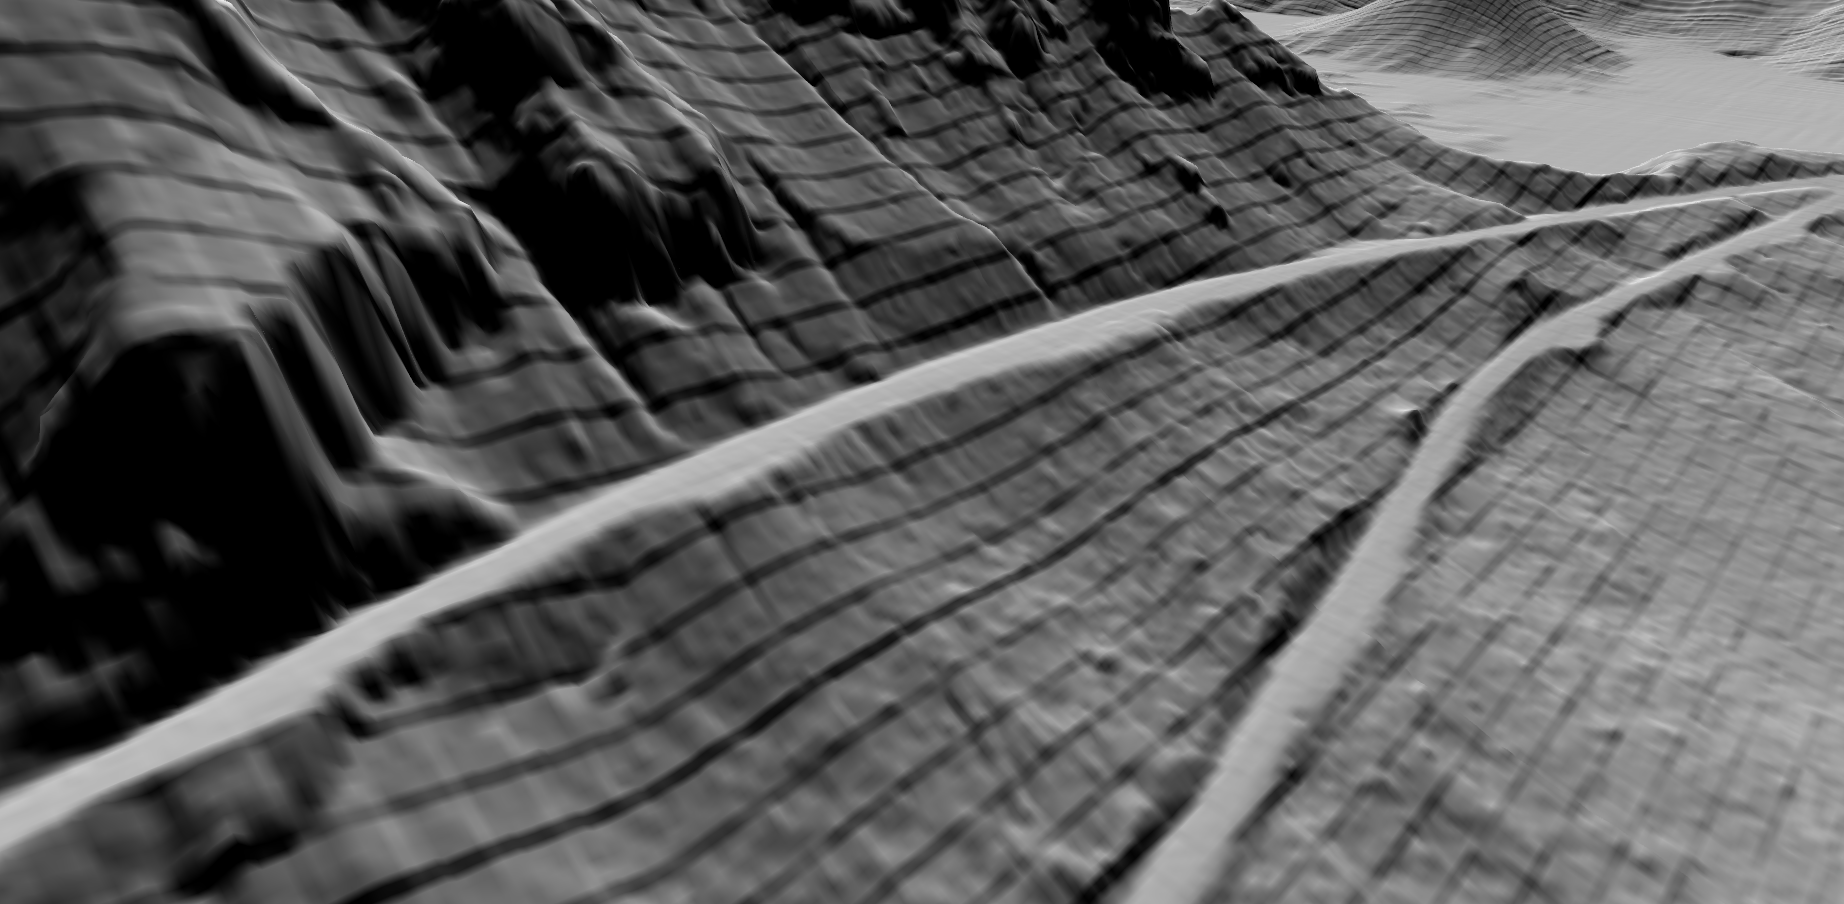
\includegraphics[scale=0.15]{craterlake_highres_zoom.png}
    \caption{A view of the level of detail on the 1m resolution DEM of the Crater Lake area}
    \label{fig:craterlake_1m_zoom}
\end{figure}

\subsubsection{DEMs with 30m and 90m Resolution} \label{dem30m90m}
NASA SRTM data for much of the world is publicly available with approximately 30 meter resolution \cite{jpl13}, and for even more of it with 90m resolution \cite{nasa00}. Due the wide availability of DEMs at these resolutions they will be used for the purposes of tracking. Figures \ref{fig:craterlake_30m} and \ref{fig:craterlake_90m} show QGIS \cite{qgis} renderings providing an overview of the DEMs with 30m and 90m resolutions respectively. 

\begin{figure}[ht]
    \centering
    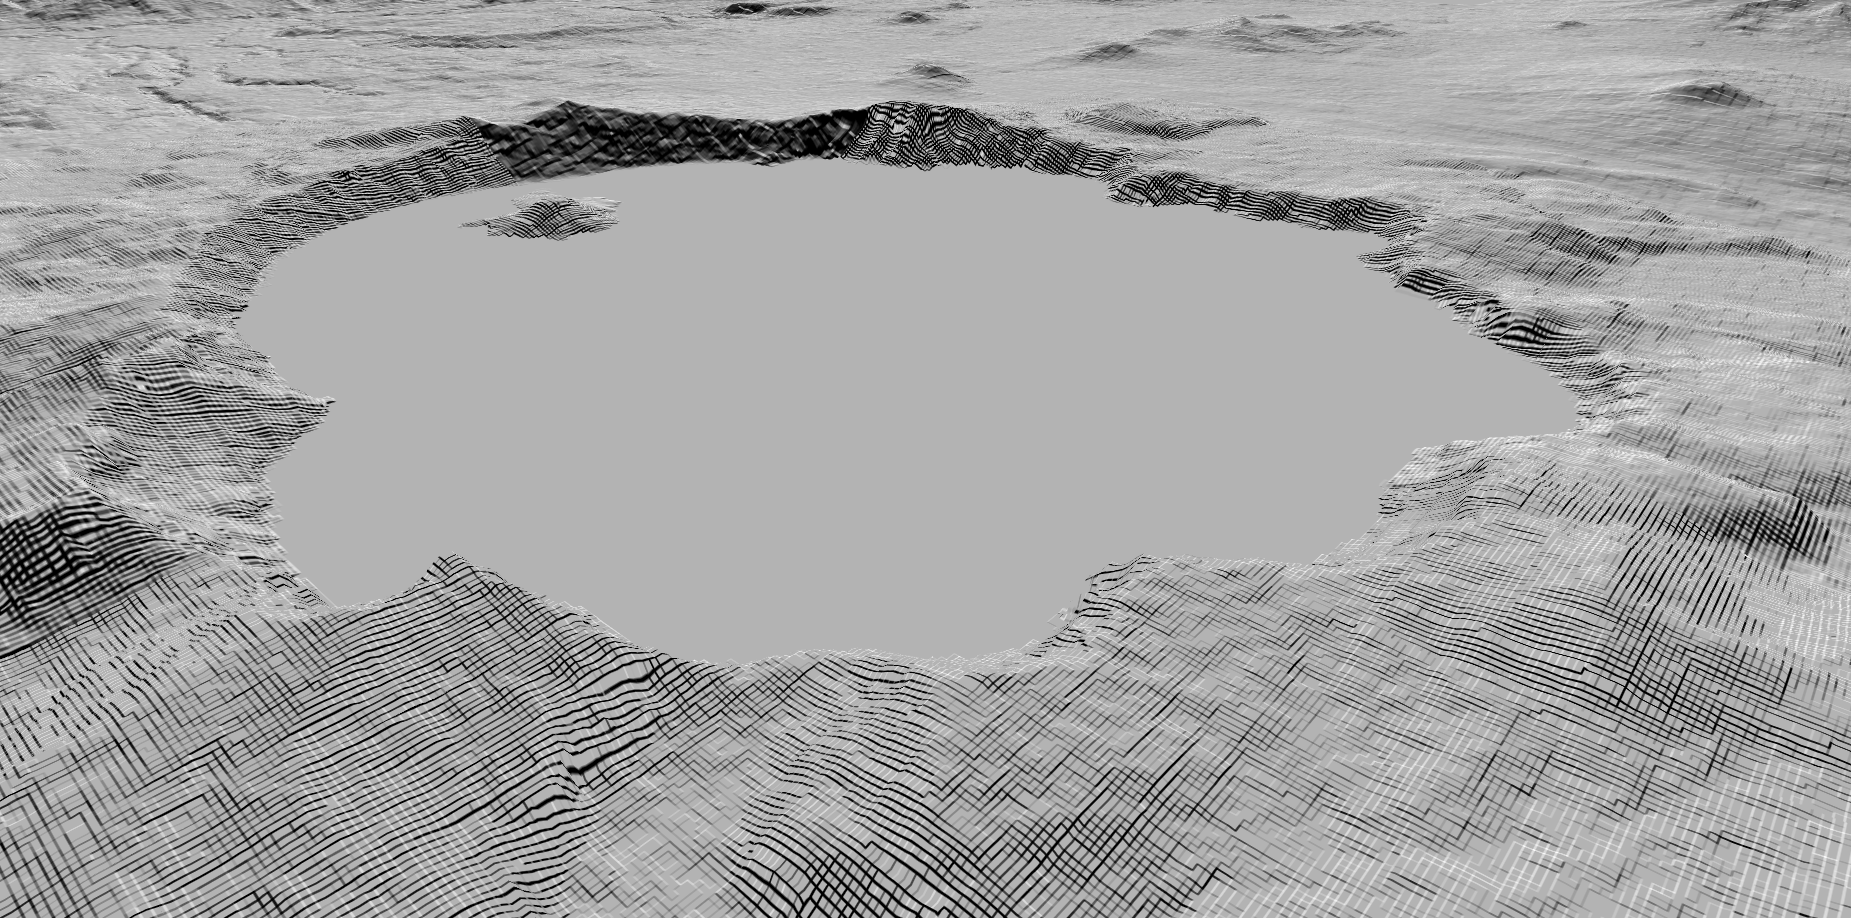
\includegraphics[scale=0.15]{craterlake_30m.png}
    \caption{The Crater Lake area visualized using the DEM with 30m resolution}
    \label{fig:craterlake_30m}
\end{figure}

\begin{figure}[ht]
    \centering
    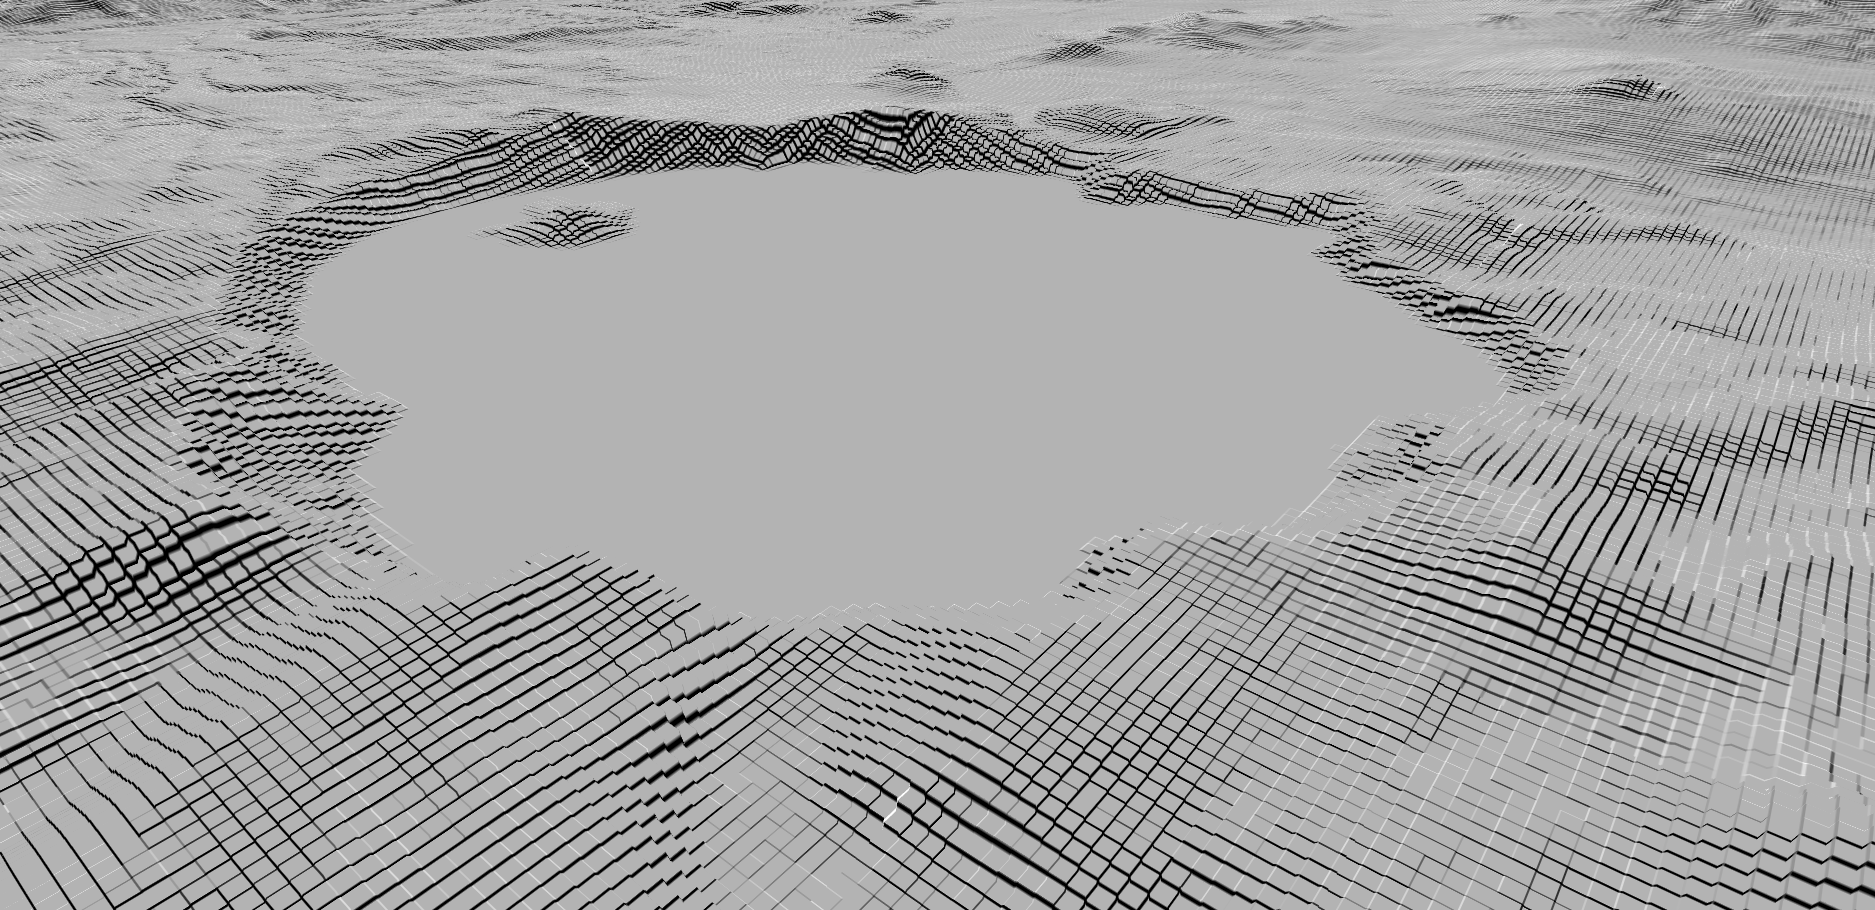
\includegraphics[scale=0.15]{craterlake_90m.png}
    \caption{The Crater Lake area visualized using the DEM with 90m resolution}
    \label{fig:craterlake_90m}
\end{figure}

\subsubsection{Corrected DEMs with 30m and 90m Resolution}
Corrected DEMs were created based on each of the 30m and 90m resolution DEMs. These corrected DEMs retained the same resolution as the models they were based on, but the elevation at each post was corrected to match the true (1m) DEM. These DEMs are intended to provide an upper bound on tracking performance using a DEM of that resolution to give some idea of how much improvement can be obtained by fixing or estimating the post heights.

\subsection{Sensor and Target Trajectories}
The sensor moves following an aerial trajectory with a constant velocity model with independent zero-mean Gaussian process noise. The target also follows a constant velocity model with independent zero-mean Gaussian process noise, but it is traveling along the ground as determined using the true terrain model. Trajectories of both types are generated independently for each Monte carlo run.

\subsection{Results} \label{results}
Performance was evaluated for all the trackers in terms of track accuracy (residual Euclidean error and RMSE), track probability of detection (TPD), and number of false tracks (NFT). An overall summary of the results (averaged over all time points in the simulation) is given in table \ref{tab:perfeval_summary}. Broadly speaking the GMM-K6-EM tracker formed fewer tracks (both true and false) than the other trackers, having the lowest NFT but also the lowest TPD and highest track error metrics in all scenarios. The trackers using a Gaussian mixture measurement model with a dynamically selected number of components (GMM-DK-SMC and GMM-DK-EM) performed similarly to one another across all metrics, which is expected since they result in a very similar measurement distribution under most conditions. These trackers consistently outperformed the baseline Gaussian measurement tracker in terms of track accuracy, with similar performance in terms of NFT and TPD. When using the corrected DEMs these trackers consistently performed the same or better than the baseline.

With the uncorrected DEMs the NFT was slightly increased for the GMM trackers with dynamically selected number of components when compared with the baseline which is of course undesirable, even though the magnitude of the increase is small. This can be explained by considering how each of the trackers will handle true detections that occur with a multimodal distribution. In these cases the GMM trackers will initialize and propagate hypotheses based on the false mode(s) as well as the true mode, while the Gaussian tracker will do so based on a Gaussian approximation of the distribution. While the modal ambiguity in the trackers using GMM measurements is resolved using MHT, it may appear at some instances that the track based on the false mode is more likely, therefor it will appear in the global hypothesis instead of the track based on the true mode. In some cases this results in the track error being large enough to not be associated with the truth, resulting in a false track. Comparatively the Gaussian measurement model may associate with the existing track and pull it off course, but may still be associated with the truth and not produce a false track. In this way the performance penalty of misleading multimodal measurements is shifted to the NFT metric for GMM trackers, while it is shifted to the track error metrics for the Gaussian tracker. With the corrected DEMs the GMM trackers instead show a slight improvement in terms of NFT, suggesting that the problem is primarily a result of inaccuracy in terrain elevation, which is assumed to be accurate by the proposed methods.

As expected correcting the DEMs resulted in improved performance for all trackers across all metrics. This suggests a direction for future work in developing a method that alleviates the assumption of accurate terrain data. This could allow for performance results somewhere in the middle of the those seen here for the uncorrected and corrected DEMs. Since a corrected DEM is not generally available, it would be desirable to obtain such results using the uncorrected DEM. One possible approach could be implemented during the sampling phase. Instead of sampling from just the measurement distribution, the distribution of the terrain data could also be sampled. Care would need to be taken to design such an approach in a way that remains computationally feasible while obtaining reasonable coverage of the sample space.

Interestingly the performance for all trackers across all metrics was actually better for the DEMs with 90m resolution than the ones with 30m resolution, but this may not be the case under all tracking conditions. In the simulated scenarios the majority of samples from the measured distribution that are not actually located near the target (i.e. belonging to the false mode for a multimodal distribution) end up on a peak located between the sensor and the targets' true position (see figure \ref{fig:sample_frame} for an example of this). The 90m DEMs can reduce the prevalence of peaks (both high and low) when compared with the 30m DEMs due to the smoothing of the area between posts that occurs, so in this scenario the result is a performance improvement. One could imagine that if the targets were instead located on this peak, the 90m DEMs could potentially reduce performance through the same smoothing effect compared with the 30m DEMs. This underscores the situational nature of the task of choosing an optimal tracking approach.

\begin{table}[ht]
\begin{center}
\small\addtolength{\tabcolsep}{-0.5pt}
\begin{tabular}{ |l|c|c|c|c| } 
 \hline
 
 \hline
 \multicolumn{5}{|c|}{30m} \\
 \hline
  & Gaussian & DK-SMC & DK-EM & K6-EM \\
 \hline
 Res. (m) & 110.779 & {\color{green}79.081}\eggplant & {\color{green}79.312} & {\color{red}112.403}\skull \\
 RMSE (m) & 149.584 & {\color{green}114.256}\eggplant & {\color{green}114.349} & {\color{red}151.696}\skull \\
 NFT & 1.884 & {\color{red}1.912}\skull & {\color{red}1.908} & {\color{green}0.840}\eggplant \\
 TPD & 0.642 & {\color{green}0.645}\eggplant & {\color{green}0.645}\eggplant & {\color{red}0.506}\skull \\
 \hline
 
 \hline
 \multicolumn{5}{|c|}{30m (corrected)} \\
 \hline
  & Gaussian & DK-SMC & DK-EM & K6-EM \\
 \hline
 Res. (m) & 75.046 & {\color{green}58.186} & {\color{green}57.645}\eggplant & {\color{red}98.854}\skull \\
 RMSE (m) & 108.069 & {\color{green}83.162} & {\color{green}82.243}\eggplant & {\color{red}138.781}\skull \\
 NFT & 1.823\skull & {\color{green}1.820} & {\color{green}1.808} & {\color{green}0.845}\eggplant \\
 TPD & 0.700 & {\color{green}0.703}\eggplant & {\color{green}0.703}\eggplant & {\color{red}0.568}\skull \\
 \hline
 
 \hline
 \multicolumn{5}{|c|}{90m} \\
 \hline
  & Gaussian & DK-SMC & DK-EM & K6-EM \\
 \hline
 Res. (m) & 95.037 & {\color{green}75.937} & {\color{green}75.146}\eggplant & {\color{red}107.485}\skull \\
 RMSE (m) & 130.094 & {\color{green}107.255} & {\color{green}105.862}\eggplant & {\color{red}140.291}\skull \\
 NFT & 1.852 & {\color{red}1.871}\skull & {\color{red}1.868} & {\color{green}0.831}\eggplant \\
 TPD & 0.689 & {\color{green}0.690}\eggplant & {\color{green}0.690}\eggplant & {\color{red}0.547}\skull \\
 \hline
 
 \hline
 \multicolumn{5}{|c|}{90m (corrected)} \\
 \hline
  & Gaussian & DK-SMC & DK-EM & K6-EM \\
 \hline
 Res. (m) & 71.507 & {\color{green}56.742} & {\color{green}55.213}\eggplant & {\color{red}96.140}\skull \\
 RMSE (m) & 102.471 & {\color{green}83.051} & {\color{green}80.821}\eggplant & {\color{red}135.656}\skull \\
 NFT & 1.820\skull & {\color{green}1.819} & {\color{green}1.809} & {\color{green}0.837}\eggplant \\
 TPD & 0.709 & {\color{green}0.710}\eggplant & 0.709 & {\color{red}0.576}\skull \\
 \hline
 
 \hline
\end{tabular}
\end{center}
\caption{Summary of performance evaluation results for all DEMs and measurement models. Lower values are better for all metrics except TPD. The best tracker for each metric is marked with \eggplant\ while the worst is marked with \skull.}
\label{tab:perfeval_summary}
\end{table}

It may also be of interest to consider the performance of each tracker at each time point during the simulation period. Figure \ref{fig:combined_rmse_plots} shows the average residual error over time, while figure \ref{fig:combined_nft_plots} shows the average number of false tracks over time. Clearly the conditions of the scenario vary over time.

At the start of the simulation period the targets are both traveling through reasonably consistent terrain with a sufficiently high grazing angle, resulting in a measurement distribution that is usually essentially unimodal. At this time the GMM trackers with dynamically selected number of components are equivalent to the Gaussian tracker since they will have just one component nearly all of the time. This equivalence can be seen in their performance results during this time period. The GMM tracker with 6 components results in a significant overfit of the measurement distribution during this period, and the resulting performance degradation can be seen in terms of track accuracy (when interpreting the reduction in NFT it is important to remember that this tracker also has a significantly lower TPD).

At around $t = 100$ the tracking conditions become more difficult as the targets become enter peaky terrain and are observed from a lower grazing angle, resulting in a multimodal measurement distribution most of the time. During this period of time the performance of the Gaussian tracker diverges from that of the GMM trackers with dynamic selection of the number of mixture components, which is now usually selected to be greater than one. It can be seen that these trackers are able to maintain a more accurate track for a longer period of time as the tracking conditions worsen when compared to the baseline Gaussian tracker, while NFT remains largely similar. During this period of time the GMM-K6-EM tracker is less of an overfit than it was when the measurement distribution was unimodal. As such the accuracy degradation of this tracker when compared with the GMM trackers that dynamically select the number of components is not as significant, but is still notable.

Eventually (around $t = 200$) the tracking conditions become very difficult as the targets remain in difficult terrain and also become occluded by terrain for a significant portion of the time. During this period all trackers struggle to maintain a consistent and accurate track. It is also during this time that the differences in NFT between trackers and between the different DEMs is most interesting. Consider the period approximately between $t = 205$ and $t = 220$, where the GMM-DK-EM tracker maintains a lower number of false alarms than the other (broadly well-performing) trackers if the corrected DEMs are used, suggesting that in some cases this tracker can reduce NFT when the terrain data is correct. Another interesting observation can be made approximately between $t = 260$ and $t = 300$ when looking at the 30m DEMs. The uncorrected 30m DEM at this time seems to be quite misleading, resulting in a notably larger number of false tracks for all trackers when compared with the corrected 30m DEM. This is especially prevalent for the GMM trackers with dynamic selection of the number of components, which may be more overconfident in the tracks they form due to their greater leveraging of misleading terrain data near the targets' positions during this period. This further supports earlier motivation for future work in developing a sampling method for determining the terrain-aided measurement distribution that does not assume the terrain data to be correct. This seems to be more important when a Gaussian mixture distribution is assumed, but could also result in improvements when assuming a Gaussian distribution.

\begin{figure}[ht]
    \centering
    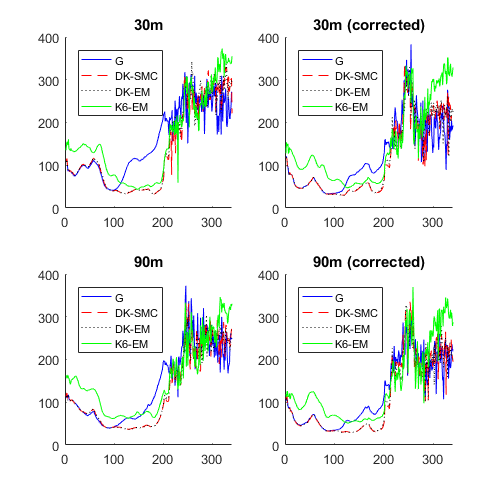
\includegraphics[scale=0.7]{combined_rmse_5000mc.png}
    \caption{Residual error (meters) over time for the 4 tracking DEMs with varying resolution and accuracy}
    \label{fig:combined_rmse_plots}
\end{figure}

\begin{figure}[ht]
    \centering
    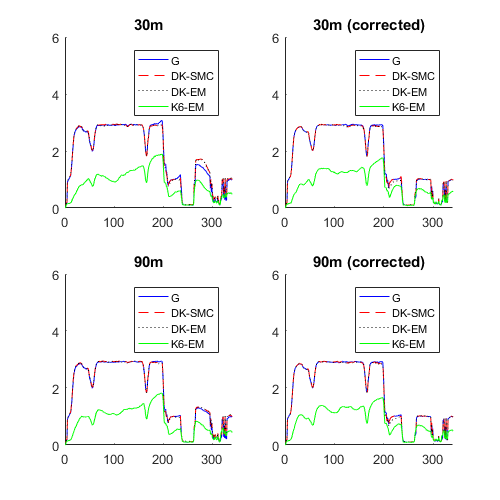
\includegraphics[scale=0.7]{combined_nft_5000mc.png}
    \caption{Number of false tracks over time for the 4 tracking DEMs with varying resolution and accuracy}
    \label{fig:combined_nft_plots}
\end{figure}

\subsection{Computation Time}
One of the objectives for the proposed algorithm, outlined in section \ref{introduction}, is that it should be usable in real-time. To determine if this has been achieved each algorithm was timed during 200 Monte Carlo runs using both 30m and 90m resolution DEMs. The timed computations included the parameterization of the terrain-aided measurement distributions for all true detections and false alarms, as well as tracking using MHT to resolve both association ambiguity and ambiguity among the mixture components (where applicable). This means that the whole online tracking process except for the detection stage (which is assumed to have already been performed and is the same for all trackers) has been timed. All timing was carried out using an Intel Core i7-6700HQ CPU running on a single thread. The average computation time (wall time) for each tracker for a simulation of 340 frames as well as the corresponding computation rate in frames per second (FPS) are given in table \ref{tab:computation_time}.

\begin{table}[ht]
\begin{center}
\small\addtolength{\tabcolsep}{-0.5pt}
\begin{tabular}{ |l|c|c|c|c| } 
 \hline
 \multicolumn{5}{|c|}{30m} \\
 \hline
  & Gaussian & DK-SMC & DK-EM & K6-EM \\
 \hline
 Time (s) & 24.546 & 28.018 & 27.734 & 25.682 \\
 FPS & 13.943 & 12.210 & 12.338 & 13.354 \\
 \hline
 
 \hline
 \multicolumn{5}{|c|}{90m} \\
 \hline
  & Gaussian & DK-SMC & DK-EM & K6-EM \\
 \hline
 Time (s) & 15.613 & 17.628 & 16.986 & 16.611 \\
 FPS & 23.779 & 20.830 & 21.640 & 22.187 \\
 \hline
\end{tabular}
\end{center}
\caption{Summary of computation times (wall time) and rates for each DEM resolution and tracker.}
\label{tab:computation_time}
\end{table}

It is expected that the GMM trackers will have longer computation time when compared with the Gaussian tracker. This is expected for two reasons. Firstly, computing the parameters for the Gaussian measurement distribution is relatively straightforward, requiring only the calculation of the sample mean and sample covariance, unlike the Gaussian mixture measurements. Secondly, the Gaussian will always result in only one additional hypothesis per measurement to consider associating with each existing track, while each Gaussian mixture measurement may result in more than one association to consider. As expected, the Gaussian tracker had the lowest computation time in simulations. When comparing the Gaussian mixture trackers the same two factors are considered (the amount of time it takes to compute the distributions parameters and the amount of time it takes to perform tracking).

Consider the computation of the distribution parameters. Both the GMM-DK-SMC and GMM-DK-EM trackers start by employing the proposed image processing methods to cluster samples and estimate the number of mixture components, while the GMM-K6-EM tracker skips this step entirely. The GMM-DK-EM and GMM-K6-EM trackers then both use EM to compute the final mixture parameters, so it is expected that latter will have an overall lower computation time for the distribution parameters. The GMM-DK-SMC tracker instead uses the cluster sample mean and sample covariance when computing the distribution parameters, which the same process at the Gaussian distribution but for each cluster and depends on the number of samples used to estimate the distribution. Based on this, the computation time for this step is expected to be similar to the same step for the Gaussian distribution (not including the image processing previously mentioned).

Less straightforward is the consideration of the amount of computation time spent performing tracking. The main factor for MHT tracking is the number of hypotheses being maintained. New measurements using the GMM trackers will generate one new hypothesis for each mixture component to consider for each existing hypothesis. The GMM-DK-SMC and GMM-DK-EM trackers will have one or more mixture components but in the simulated scenario the number of mixture components rarely exceeded 2, and was frequently 1. The GMM-K6-EM tracker always uses 6 mixture components. Initially one might expect then that the GMM-K6-EM tracker would take the longest time during the tracking phase, but it is also important to consider that an MHT tracker uses pruning to reduce the number of hypotheses by removing those that have a low track score. Recall that in section \ref{results} it was noted that the GMM-K6-EM tracker formed fewer tracks overall than all other trackers, despite the larger number of mixture components. This suggests that many of the hypotheses generated by this tracker are quickly deemed unlikely and are pruned from the hypothesis tree.

Examining the measured total computation time for each of the GMM trackers, the results are largely as expected. The GMM-K6-EM tracker skips the image processing step and forms fewer tracks, and has a lower computation time than the other GMM trackers. Comparing computation time of the GMM-DK-SMC and GMM-DK-EM trackers (which have the same number of mixture components and form a very similar number of tracks) should indicate which method is faster to compute the final distribution parameters, which seems to be EM in this case despite the fact that EM is an iterative method that depends on the number of samples as well as the number of iterations. However the cluster sample mean and sample covariance implementation was created for the purposes of these simulations, while the EM implementation is an open source implementation that is highly optimized (described in detail in \cite{sanderson2017open}). In light of this, such a result is not entirely unexpected.

Lastly, increasing the resolution of the DEM (30m post spacing compared with 90m) is expected to result in increased computation time. This is because more cells of the DEM need to be traversed before reaching the point of intersection during sampling (see section \ref{surfaceintersections}). The results observed are consistent with this expectation. Similar performance differences between trackers can be observed on both DEMs. If DEM resolution is very high, computational cost may become prohibitive.



\section{Conclusion} \label{conclusion}
This paper considers the problem of terrain-aided tracking of ground targets from an aerial platform using a sensor that provides only angular measurements of the position of a target (such as a camera). Previous works assume the measurement distribution to be Gaussian, which fits conveniently into most existing tracking frameworks. As identified in \cite{collins1989terrain,collins1998using,davison1999mobile}, the actual measurement distribution may be multimodal under some operational conditions. To address this mismatch this paper proposes to model the measurement distribution as a Gaussian mixture distribution. A framework is proposed for terrain-aided tracking of multiple targets using Multiple Hypothesis Tracking (MHT) to resolve ambiguities both in measurement-to-track association as well in which mode of the multimodal measurement distribution best represents the location of the target. The latter is achieved using a similar method to those employed in \cite{li2013multitarget,yamada2017multi}, where each mode of the measurement distribution corresponds to a Gaussian hypothesis allowing tracking to be conducted in the normal way for each hypothesis.

Existing algorithms such as Expectation Maximization (EM) allow for parameterization of a Gaussian Mixture distribution based on a set of samples, but these methods require the number of mixture components to be known or estimated independently. One possibility is to simply assume a relatively large fixed number of components, resulting in an overfit of the samples. Unfortunately this may not result in well-spaced components that can be effectively split into different hypotheses for tracking purposes. This paper presents a method for estimating the number of mixture components in the context of terrain-aided tracking based on clustering of samples using morphological image processing techniques. Following the proposed clustering step the distribution parameters can be computed using either the sample mean and sample covariance of each cluster, or by using the EM algorithm.

Simulations were conducted to evaluate and compare the tracking performance using the proposed Gaussian mixture measurement distribution against existing methods assuming a Gaussian measurement distribution. Three different methods for computing the parameters of a Gaussian mixture measurement models were considered. Two of the methods used the proposed clustering method to estimate the number of mixture components, followed by computation of the final distribution parameters using either cluster sample mean and sample covariance (in GMM-DK-SMC) or EM (in GMM-DK-EM). The final method under consideration (GMM-K6-EM) assumed a distribution with 6 components and used EM to parameterize the distribution. All methods were evaluated using 4 different tracking DEMs with varying resolution and accuracy.

Performance was evaluated in terms of track accuracy (residual error and RMSE), track probability of detection (TPD), and number of false tracks (NFT). Both trackers using the proposed image processing method performed similarly across all metrics in all scenarios, with one of these trackers consistently providing the best residual error, RMSE, and TPD among all trackers evaluated. The most substantial improvements were in terms of track accuracy. Comparing these trackers with the Gaussian baseline in terms of NFT, the results depend on the accuracy of the DEM. For the corrected DEMs these trackers also slightly improved NFT, but for the uncorrected DEMs there was a slight degradation in terms of this metric. This is likely due to the fact that the uncorrected DEMs are providing misleading information, which is not accounted for when sampling the measured target position distribution (at which time the terrain data is assumed to be correct). The GMM tracker that did not use the proposed image processing methods had the lowest NFT due to forming fewer tracks overall, but also showed a substantial performance degradation across all other metrics.

The proposed methods offer a performance trade-off that may be favorable for use in realistic tracking applications, offering a substantial improvement in track accuracy and a slight improvement in TPD at the cost of only a slight degradation in NFT, while remaining computationally feasible. Additionally the promising results of improving across all metrics when using corrected DEMs, though not typically available in realistic conditions, suggest a direction for future work. Specifically the sampling method could be adjusted to account for uncertainty in terrain data, which may yield results somewhere between those obtained using the corrected and uncorrected DEMs without the requirement of actually having a corrected DEM.

%\tableofcontents

\bibliographystyle{IEEEtran}
\bibliography{references}
\end{document}


